\chapter{Описание предметной области и постановка задачи} \label{ch:ch1}

\section{Описание электронного документооборота} \label{sec:ch1/sec1}
Многим предприятиям, как коммерческим, так и некоммерческим требуется отлаженная схема для работы с документацией.
В эпоху цифровых технологий на смену классическому "бумажному" документообороту приходит \textbf{электронный документооборот}.
Он эффективно аккумулирует многие процессы, позволяет работать с документами и данными в электронном виде, но также обладает достаточным количеством отличительных особенностей, а именно:
 \begin{itemize}
 	\item \textbf{Экономия времени:} работникам не приходится долго искать бумажные экземпляры, все документы постоянно находятся в электронном виде и собраны в одном месте. Более того, постоянное резервное копирование системы исключает потерю или же намеренное искажение данных. Так, благодаря устройству системы обеспечивается значительная экономия времени, ресурсов, упрощается работа сотрудников.
 	\item \textbf{Оптимизация использования физического пространства и технических средств:} при переходе на электронный документооборот освобождается площадь под серверы и другое оборудование, предназначенное для хранения документов. В зависимости от статуса и актуальности информации, документы и файлы могут безопасно удаляться по истечении срока их хранения. Управление данными не только помогает соответствовать корпоративным нормам, но и способствует более адекватному использованию места для хранения.
 	\item \textbf{Снижение затрат на распечатку, почтовые марки, конверты и пересылку:} бумажные документы, которые пересылаются между отделами или поставщиками, могут пересылаться в электронном виде.
 \end{itemize}

Выше перечислены лишь немногие преимущества данного подхода к работе с документацией, но их уже достаточно для того, чтобы большинство организаций приветствовали внедрение 	систем электронного документооборота (СЭД) в свои экосистемы.

Такая система может быть построена на основе следующих технических решений:
\begin{itemize}
	\item Централизованная база данных.
	\item Распределённые хранилища.
	\item Документо-ориентированный блокчейн.
\end{itemize}
\section{Обзор существующих решений} \label{subsec:ch1/sec2}
Для обзора возьмем несколько самых популярных СЭД в России:
\begin{itemize}
	\item DIRECTUM.
	\item DocsVision.
	\item TESSA.
	\item ТЕЗИС.
\end{itemize}
Итак, о каждой по порядку.

СЭД «ТЕЗИС» — это программное обеспечение, написанное на языке Java. Оно базируется на платформе CUBA, особенности которой позволяют масштабировать систему, делают ее надежной и отказоустойчивой. Данная платформа используется для быстрого и простого создания различного корпоративного ПО, но создание на ее базе СЭД – это особый случай. CUBA, прежде всего, являет собою платформу с открытым кодом, которая поддерживается объединениями разработчиков по всему миру. Создателем CUBA является российская компания Haulmont, которая уже представила свои достижения на международном уровне и получила соответствующее признание. Важно то, что Java – это распространенный язык для корпоративных решений, существует достаточно много специалистов с необходимым уровнем квалификации, благодаря чему представляется возможной дальнейшая поддержка данного программного решения. 

Также «ТЕЗИС» удобна тем, что она предоставляет разработчикам инструменты для создания дополнительных компонентов, расширения функционала и свободного масштабирования системы. Корпоративные разработчики могут напрямую переопределять функции, классы, вносить необходимые изменения в код программного обеспечения и подстраивать его под свои нужды. 

Отличительной особенностью является отсутствие десктопного клиента, присутствует только веб-интерфейс, через который также производится работа администратора. Стоит заметить, что многие корпоративные решения строятся именно на веб-клиентах, а их использование зачастую не вызывает каких-либо проблем. Громоздкие, объемные десктопные клиенты наоборот могут быть проблемой из-за сложности из разворачивания и настройки. Веб-клиент экономит силы и ресурсы команды разработчиков, упрощает работу с клиентом.

Следующее решение – это «DocsVision», это программное обеспечение, имеющее достаточно много версий и длительную историю. Последняя версия ПО строится на основе новой и удобной платформе, что обеспечивает преемственность и не только. Кроме того, в данной СЭД имеется продуманная, удобная структура хранения данных, имеются ориентированные на пользователя инструменты для работы с базами данных. Программное решение имеет клиенты для разных операционных систем. 

У этой системы есть и свои недостатки, например, преимущественная ориентированность на Windows, полная привязка к этой платформе. Разработчики анонсировали поддержку полного спектра платформ. Система также требовательна к аппаратным ресурсам, слабые системы не позволят его эффективно использовать. 

СЭД «TESSA» является еще одним современным и эффективным решением. Данное ПО разработано для Windows, оно не имеет дополнительных унаследованных модулей и компонентов, что делает СЭД простой, динамичной и удобной. Здесь нет десктопного клиента, имеется лишь веб-интерфейс, система имеет огромный потенциал и возможности. Имеются и определенные недостатки, среди которых упомянутое исключительное ориентирование на Windows, что затрудняет использование этого решения в ряду случаев. Разработчик уже анонсировал поддержку других платформ, которая будет реализована в будущем, при правильной реализации и сохранении подхода разработчику удастся вывести «TESSA» на новый уровень.  

СЭД «ДЕЛО» в первую очередь ориентирована на пользователя, ее интерфейс прост и интуитивно понятен. Программное решение в достаточной мере соответствует требованиям MoReq. Изначально разработчик создавал свое решение для ОС Windows, но в дальнейшем была реализована поддержка и других платформ, что делает данный продукт сравнительно более зрелым и удобным. Так, при необходимости разработчик обеспечивает реализацию решения на стеке Linux/PostgreSQL. 

Архитектура СЭД строится на основе подхода «клиент-сервер», но на данный момент она скорее является трехкомпонентной, что также вносит свои коррективы в использование и развитие СЭД. Большая часть компонентов и кода этого ПО унаследованы, а потому реализация новых решений и другой архитектуры – это сложное и неоправданное с экономической точки зрения решение. Стоит заметить, что данная СЭД на протяжении длительного периода времени являлась лидером на рынке, но на данный момент существует достаточно конкурентоспособных и качественных аналогов. 

Последнее решение – это СЭД «Directum», которая также имеет проработанный и ориентированный на пользователя интерфейс, удобные инструменты для работы, также разработчик частично геймифицировал программное обеспечение, позволил интегрировать его в другие системы и не только. Благодаря этому использовать «Directum» просто, удобно, чем и пользуются многие компании в корпоративном пространстве. 

Несмотря на такую ориентированность на пользователя, СЭД не является достаточно технологичной, у нее есть свои недостатки. Прежде всего, разработчик использует собственный инструментарий, а также язык программирования ISBL, что привносит определенные риски. Так, развитие ПО возможно исключительно благодаря корпоративным клиентам, а также партнерам разработчика. ISBL наследует основы Delphi, а потому он не является столь популярным и массовым, его поддержка затруднена отсутствием большого количества квалифицированных кадров. 

Данная СЭД строго привязана к ОС Windows. Стоит заметить, что эта система входит в реестр Минкомсвязи, но это не повышает конкурентоспособность программного обеспечения, что также обуславливается популяризацией Linux. Это тенденция, которая не только способствует экономии, но и ускоряет разработку, упрощает использование СЭД и не только, но платформы с закрытым программным кодом не дают свободно добиться этого. 


\section{Описание используемых технологий} \label{sec:ch1/sec3}

\subsection{Описание фреймворка Hyperledger Fabric} \label{subsec:ch1/sec3/subsec1}
Технологии блокчейна первоначально приобрели популярность, поскольку они рассматривались как способ избавиться от посредника и децентрализовать систему. С тех пор блокчейн стал свидетелем растущего интереса со стороны разных вариантов использования. Блокчейн - это общий распределенный реестр, который регистрирует транзакции и поддерживается несколькими узлами в сети, где узлы не доверяют друг другу. Каждый узел содержит идентичную копию реестра, которая обычно представляется в виде цепочки блоков, причем каж­ дый блок представляет собой логическую последовательность транзакций. Такой блок заключает в себе хеш своего предыдущего предыдущего блока, тем самым гарантируя неизменность регистра. Блокчейн часто называют новым поколени­ ем систем баз данных, по сути являющимся распределенной системой обработки транзакций, в которой узлам не доверяют, и системе необходимо достичь византий­ ской отказоустойчивости. Блокчейн обеспечивает сериализуемость, неизменность и криптографическую верификацию без единой точки доверия в отличие от систе­мы баз данных; свойства, которые вызвали принятие блокчейна в самых разных отраслях промышленности.


Блокчейн сети могут быть публичными (Permissionless), либо частными (Permissioned). В сети без прав доступа или в публичной сети, такой как Bitcoin или Ethereum, любой может присоединиться к сети для выполнения транзакций. Из-за большого количества узлов в общедоступной сети для согласования транзак­ций и создания блока используется подход, основанный на доказательстве работы. В приватной сети идентификация каждого участника известна и подтверждена криптографически, так что блокчейн может хранить информацию о том, кто выполнил какую транзакцию. Кроме того, в такой сети могут быть встроены ши­рокие механизмы контроля доступа, чтобы ограничить круг лиц, которые могут
\begin{itemize}
	\item считывать и добавлять данные в реестр,
	\item проводить транзакции,
	\item управлять участием в сети блокчейнов.
\end{itemize}
Приватная сеть хорошо подходит для корпоративных приложений, которые требуют аутентифицированных участников. Каждый узел в приватной сети может принадлежать различным организациям. Кроме того, корпоративные приложения нуждаются в сложных моделях данных и операциях, которые могут поддерживаться с помощью смарт-контрактов. Предприятия ценят возможность интеграции разнородных систем без необходимости создания централизованного решения и обеспечения уровня доверия между недоверяющими сторонами или привлечения доверенной третьей стороны. Trade Finance и Food Safety являются примерами приложений блокчейна, где участники видят ценность в преимуществах наглядности, которые распределенный реестр предлагает по сравнению с существующими слабосвязанными централизованными системами. Существует большое беспокойство по поводу производительности приватных платформ блокчейна и их способности обрабатывать огромный объем транзакций с низкой задержкой. Другой проблемой является богатство языка для описания транзакций. Различные платформы блокчейна, такие как Quorum, Corda, решают эти проблемы, используя различные методы, полученные из области распределенных систем. Hyperledger Fabric является платформой корпоративного уровня с открытым исходным кодом, которая имеет модульную конструкцию и высокую степень специфики благодаря доверенным моделям и подключаемым компонентам. В настоящее время Fabric используется во многих различных случаях, таких как оцифровка глобальной торговли , SecureKey, Everledger, и является предметом нашего исследования. Fabric состоит из различных компонентов, таких как индоссанты, сервисные узлы и коммиттеры. Кроме того, он представляет собой различные этапы обработки транзакции, такие как этап подтверждения, этап проверки, этап проверки и принятия.

Hyperledger Fabric - это реализация приватной системы блокчейна, которая обладает множеством уникальных свойств, подходящих для приложений корпоративного класса. Он может выполнять произвольные смарт контракты, реализованные на языке Go / Java / Javascript. Он поддерживает определенную модель доверия приложения для проверки транзакций и подключаемый протокол консенсуса. Сеть Fabric состоит из объектов разных типов, одноранговых узлов, сервисных узлов и клиентов, принадлежащих к разным организациям. Каждый из них имеет идентификатор в сети, который предоставляется поставщиком услуг членства (MSP), обычно ассоциированным с организацией. Все объекты в сети могут видеть идентификаторы всех организаций и могут их проверять.

\subsubsection{Ключевые компоненты в Hyperledger Fabric} \label{subsubsec:ch1/sec3/subsec1/subsubsec1}

\textbf{Узел(Peer).} Одноранговый узел выполняет код, который реализует смарт-контракт пользователя и поддерживает реестр в файловой системе. Также код разрешает доступ к общему состоянию с помощью четко определенных API реестра. Одноранговый узел дополнительно выделяется как подтверждающий одноранговый узел, который имеет логику в виде кода и выполняет его для подтверждения транзакции или принимающий одноранговый узел, который не содержит логику. Независимо от этой дифференциации оба типа сверстников поддерживают регистр. Кроме того, оба одноранговых узла поддерживают текущее состояние как StateDB в хранилище значений ключей, так что код может запрашивать или изменять состояние, используя язык запросов базы данных.

\textbf{Политика одобрения (Endorsement Policies).} Скрипты написаны на языках общего назначения и выполняются на непроверенных пирах в сети. Это создает множество проблем, одна из которых заключается в недетерминированном выполнении, а другая - в доверии результатам любого данного узла. Политика одобрения решает эти две проблемы, определяя набор узлов, которым необходимо смоделировать транзакцию и подтвердить или подписать цифровым способом результаты выполнения. Политики одобрения указываются как логические выражения для идентификаторов участников сети. Участник здесь является членом конкретной организации.

Системный код имеет ту же модель программирования, что и обычный пользовательский код, но встроен в исполняемый файл узла, в отличие от пользовательского. Fabric реализует различные системы:
\begin{itemize}
	\item системы жизненного цикла (LSCC) - для установки / создания / обновления кода;
	\item системы одобрения (ESCC) - для подтверждения транзакции путем цифровой подписи ответа;
	\item системы проверки (VSCC) - для проверки подписи подтверждения транзакции, установленной в соответствии с политикой подтверждения;
	\item системы конфигурации (CSCC) - для управления конфигурациями каналов.
\end{itemize}

\textbf{Каналы.} В Fabric представлена концепция, называемая каналом, как
«частная» подсеть связи между двумя или более одноранговыми узлами для обеспечения уровня изоляции. Транзакции на канале видят только узлы и участники. Постоянный регистр и код указаны для каждого канала. Кроме того, консенсус применим для каждого канала, то есть не существует определенного порядка транзакций по каналам.
\begin{figure}[ht]
	\centering
	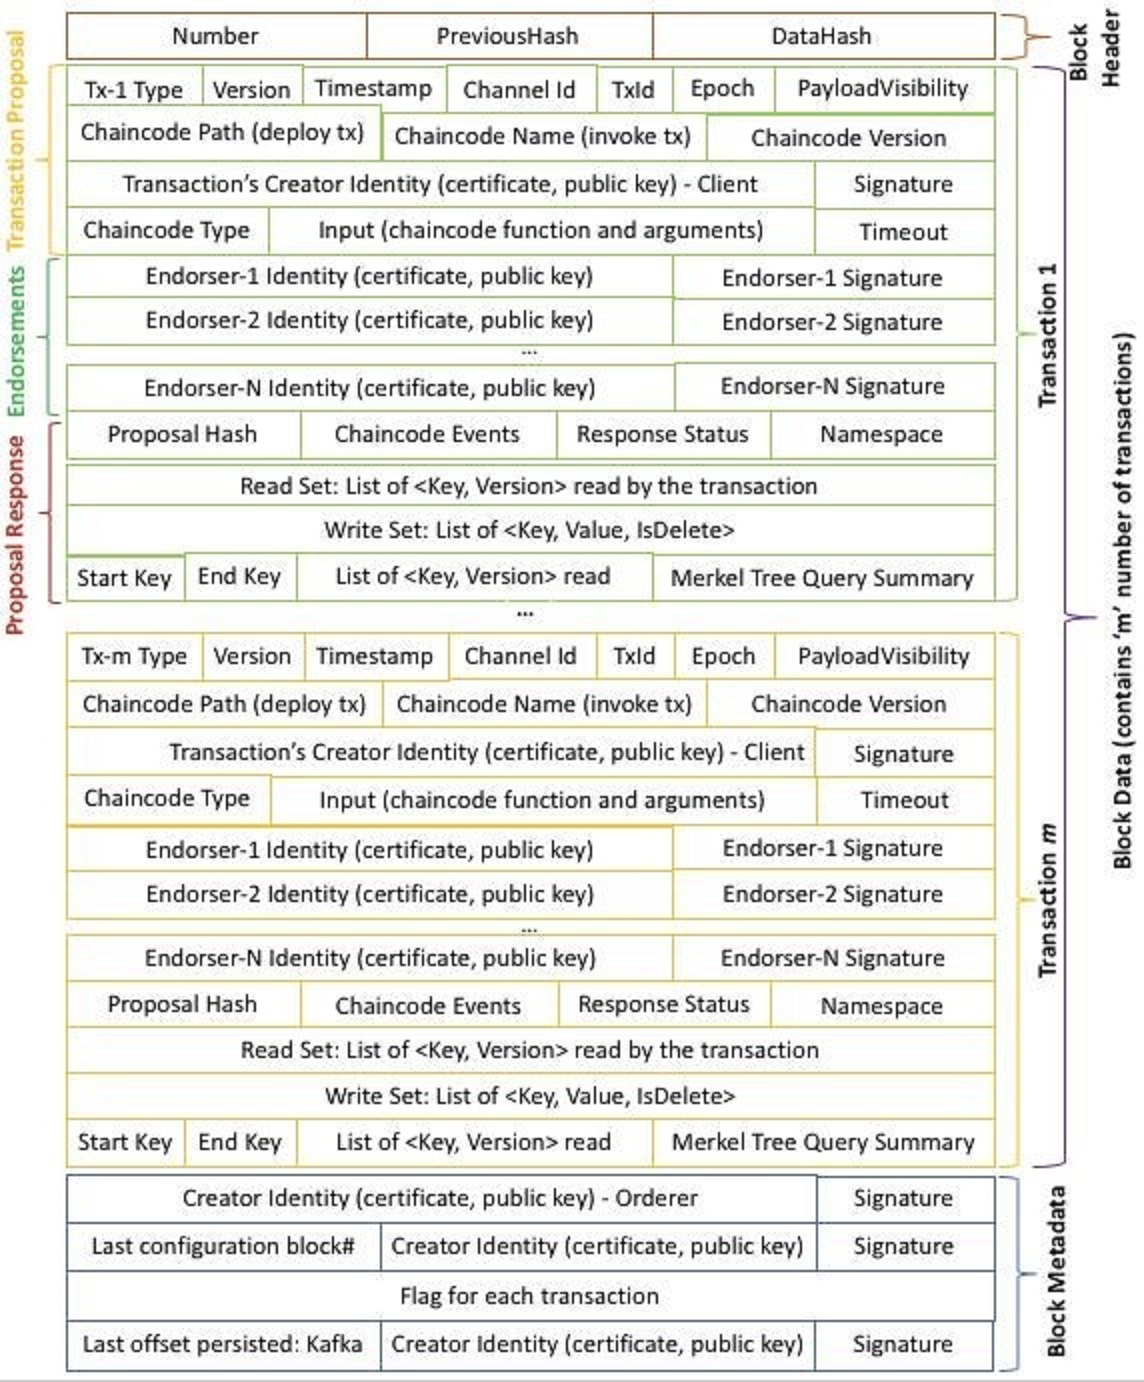
\includegraphics [scale=0.5] {hlf_block_structure}
	\caption{Структура блока Hyperledger Fabric}
	\label{fig:hlf_block_structure}
\end{figure}

\textbf{Сервисная служба (Ordering Service).} Узел сервисной службы (OSN) участвует в консенсусе и составляет блок транзакций, который доставляется узлам по протоколу “сплетни” (gossip protocol). Структура блока в Fabric показана на рисунке \ref{fig:hlf_block_structure}. Сервисная служба является модульной и поддерживает подключаемый механизм консенсуса. По умолчанию последовательное упорядочение (то есть консенсус) достигается с помощью базового кластера Kafka / Zookeeper. OSN публикуют транзакции в темах kafka и используют упорядоченный и неизменный характер записей в темах kafka для создания уникальной упорядоченной последовательности транзакций в блоке. Блок обрезается, когда добавляется максимальное количество новых транзакций с момента последнего среза блока или установленное время ожидания с момента последнего среза блока. Когда какое-либо одно условие удовлетворяется, блок доставляется на равноправные узлы.

\textbf{Клиент (Client).} Клиентское приложение отвечает за составление предложения по транзакции, как показано на рисунке \ref{fig:hlf_tx_route}. Клиент отправляет предложение по транзакции одному или более узлам одновременно для сбора ответов с одобрениями для удовлетворения политики одобрения. Затем он передает транзакцию сервисной службе, которая включит её в блок и доставит всем узлам для проверки и подтверждения. В Fabric ответственность лежит на клиенте, чтобы гарантировать, что транзакция правильно сформирована и удовлетворяет политикам одобрения.
\begin{figure}[ht]
	\centering
	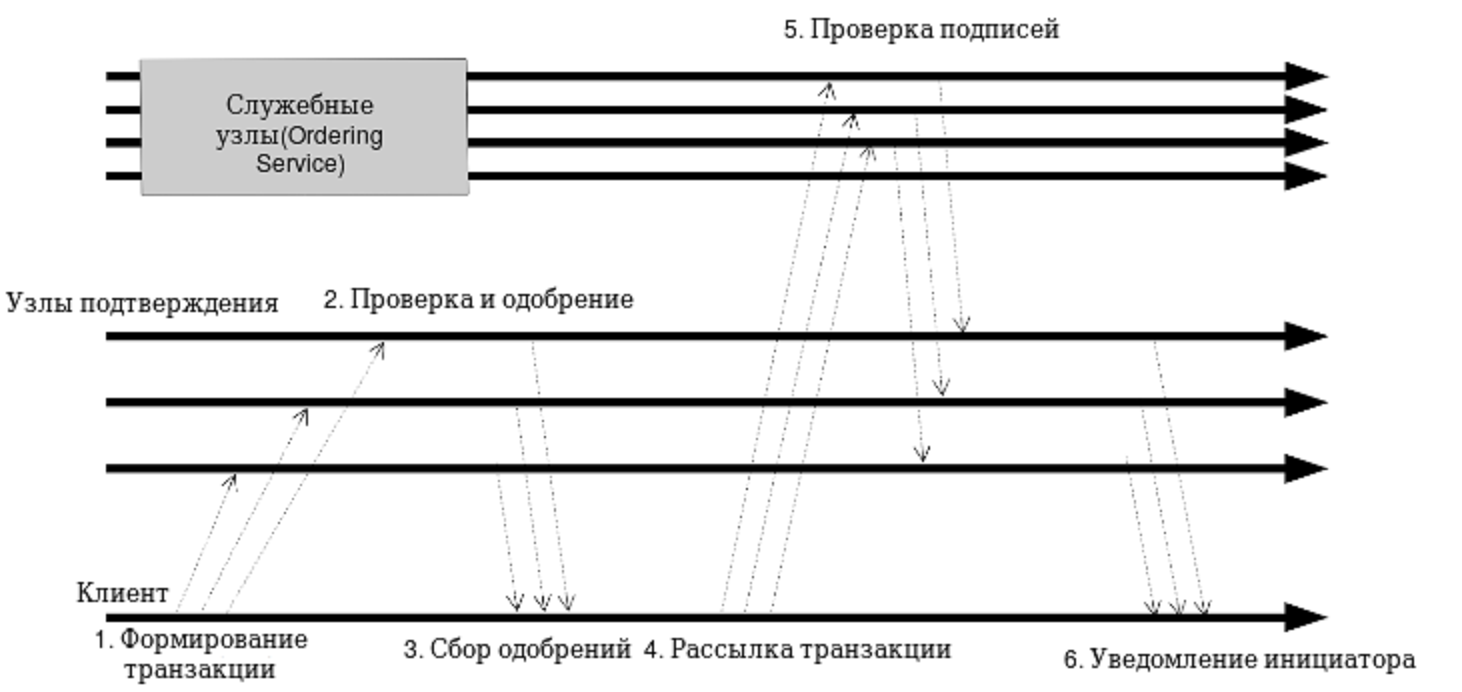
\includegraphics [scale=0.5] {hlf_tx_route}
	\caption{Путь транзакции в Hyperledger Fabric}
	\label{fig:hlf_tx_route}
\end{figure}

\subsubsection{Путь транзакции в Hyperledger Fabric} \label{subsubsec:ch1/sec3/subsec1/subsubsec2}

В отличие от других блокчейн-сетей, в которых используется модель транзакции “order-execute”, в Fabric используется модель “simulate order-validate\& commit”. На рисунке \ref{fig:hlf_tx_route} изображен поток транзакций, который включает в себя 3 этапа:
\begin{itemize}
	\item Фаза одобрения - моделирование транзакции на отдельных участниках и сбор изменений состояния;
	\item Этап	упорядочения	-	упорядочение транзакций по согласованному протоколу;
	\item Этап валидации - валидация с последующей фиксацией в реестре.
\end{itemize}

Прежде чем транзакции могут быть отправлены в Fabric, необходимо загрузить сеть с участвующими организациями, их MSP и идентификаторами для партнеров. Сначала в сети заказчика создается канал с соответствующими MSP организации. Во-вторых, коллеги каждой организации присоединяются к каналу и инициализируют реестр. Наконец, необходимые смарт-контракты устанавливаются на канал.


\textbf{Фаза одобрения (Endorsement Phase).} Клиентское приложение, использующее Fabric SDK создает предложение по транзакции для вызова функций кода, которые, в свою очередь, будут выполнять операции чтения и
/ или записи в состоянии регистра. Предложение подписывается учетными данными клиента, и клиент отправляет его одному или более подтверждающим партнерам одновременно. Политика одобрения для смарт-контракта диктует, каким организациям-партнерам клиент должен отправить предложение для моделирования.

Во-первых, каждый подтверждающий одноранговый узел проверяет, что отправитель уполномочен вызывать транзакции на канале. Во-вторых, одноранговый узел выполняет код, который может получить доступ к текущему состоянию регистра в одноранговом узле. Результаты транзакции включают в себя значение ответа, набор для чтения и набор для записи. Все операции чтения читают текущее состояние регистра, а записи перехватываются и изменяют приватное рабочее пространство транзакции. В-третьих, подтверждающий одноранговый узел вызывает системный код, называемый ESCC, который подписывает этот ответ на транзакцию с идентификатором партнера и отвечает обратно клиенту с ответом на предложение. Наконец, клиент проверяет ответ предложения, чтобы убедиться, что на нем стоит подпись партнера. Клиент собирает достаточное количество ответов на предложения от разных партнеров, проверяет, что одобрения одинаковы. Поскольку каждый узел мог выполнить транзакцию на разной высоте в блокчейне, возможно, что ответ предложения отличается. В таких случаях клиент должен повторно предоставить предложение другим партнерам, чтобы получить достаточные совпадающие ответы.

\textbf{Фаза сервиса (Ordering Phase).} Клиент передает правильно оформленное сообщение о транзакции в службу сервиса. Транзакция будет содержать наборы для чтения и записи, подписи одноранговых узлов и идентификатор канала. Узел службы сервиса не требуется проверять содержимое транзакции для выполнения своей операции. Он получает транзакции от разных клиентов для разных каналов и ставит их в очередь для каждого канала. Он создает блоки транзакций для каждого канала, подписывает блок своим ключом и доставляет их партнерам, используя протокол обмена сообщениями.

\textbf{Этап валидации (Validation Phase).} Все одноранговые, как одобряющие, так и фиксирующие узлы на канале, получают блоки из сети. Узел сначала проверяет подпись узла сервиса на блоке. Каждый действительный блок декодируется, и все транзакции в блоке проходят проверку VSCC перед выполнением проверки MVCC.

Проверка	VSCC	оценивает	одобрения	в	транзакции	в		соответствии	с политикой	одобрения,		указанной	для	смарт-контракта.		Если	политика подтверждения не выполняется, то эта транзакция помечается как недействительная. Проверка MVCC. Как следует из названия, проверка Multi-Version Concurrency Control гарантирует, что версии ключей, считанные транзакцией во время фазы подтверждения, совпадают с их текущим состоянием в реестре во время коммита. Это похоже на проверку конфликта чтения-записи, выполняемую для управления параллелизмом, и выполняется последовательно для всех действительных транзакций в блоке (как отмечено проверкой VSCC). Если версии набора для чтения не совпадают, это означает, что предыдущая транзакция изменила прочитанные данные и была (с момента одобрения) успешно принята, транзакция помечается как недействительная. Чтобы убедиться, что фантомных чтений не происходит, для запросов выполняется повторный запрос и сравниваются хэши результатов (которые также сохраняются как часть набора для чтения, полученного во время одобрения).

\textbf{Этап обновления реестра (Ledger Update Phase).} В качестве последнего шага обработки транзакций регистр обновляется путем добавления блока в локальный регистр. StateDB, которая содержит текущее состояние всех ключей, обновляется наборами записей допустимых транзакций (как отмечено валидацией MVCC). Эти обновления для StateDB выполняются атомарно для блока транзакций и применяют обновления, чтобы привести StateDB в актуальное состояние после обработки всех транзакций в блоке.

\section{Триллеммы децентрализованных систем} \label{sec:ch1/sec4}

Главная проблема распределенных архитектур описана в утверждении, общепринято известном как “теорема CAP”. Теорема CAP, постулированная Эриком Брюером в 2000 году, утверждает, что в распределенном хранилище данных невозможно гарантировать более двух из трех свойств: согласованность (Consistency), доступность (Availability) и устойчивость к разделению (Partition Tolerance). Распределенное хранилище данных, таким образом, может быть охарактеризовано только двумя свойствами, а именно CA, CP или AP. Схематично данное разделение представлено на рисунке \ref{fig:cap_theoreme}.

\begin{figure}[ht]
	\centering
	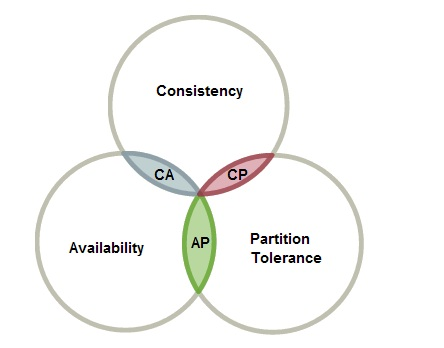
\includegraphics [scale=0.5] {cap-theorem}
	\caption{Теорема CAP}
	\label{fig:cap_theoreme}
\end{figure}

Более конкретно, теорема нацелена на распределенные системы, развернутые через ненадежные сети (сети с ошибками и задержками, такие как Интернет), приводя к разделению компонентов системы. Согласно CAP, в этих средах архитектура системы должна быть ориентирована на баланс между доступностью и последовательность. Например, ACID (атомарность, согласованность, изоляция,
стойкость), обычно предоставляемый RDBMS (реляционной базой данных) гарантирует согласованность на одном узле за счет доступности через несколько узлов (тип CP).

В отличие от этого, Fabric спроектирован так же, как и многие другие блокчейн платформы, как тип AP с возможной согласованностью, также называемой BASE (Basically Available, Soft state, Eventual consistency), при этом такой подход напрямую противопоставляется ACID. Под базовой доступностью подразумевается такой подход к проектированию приложения, чтобы сбой в некоторых узлах приводил к отказу в обслуживании только для незначительной части сессий при сохранении доступности в большинстве случаев. Неустойчивое состояние подразумевает возможность жертвовать долговременным хранением состояния сессий (таких как промежуточные результаты выборок, информация о навигации, контексте), при этом концентрируясь на фиксации только критичных операций. Согласованность в конечном счёте, трактуются как возможность противоречивости данных в некоторых случаях.

В контексте блокчейна, свойства CAP могут быть определены следующим образом:
\begin{itemize}
	\item \textbf{Согласованность:} сеть блокчейн избегает разветвлений цепи.
	\item \textbf{Доступность:} транзакции, представленные клиентами, постоянно записываются в блокчейн и доступны на всех сетевых пирах.
	\item \textbf{Устойчивость к разделению:} сеть блокчейна продолжает работать, несмотря на произвольное количество транзакций или блоков отброшенных (или задерживающихся) в физической сетевой среде между узлами.
\end{itemize}

Fabric реализует свойства CAP следующим образом:
\begin{itemize}
	\item \textbf{Согласованность:} общий порядку транзакций и управление версиями с использованием MVCC.
	\item \textbf{Доступность:} путем размещения копии блокчейна в каждом из пиров.
	\item \textbf{Устойчивость к разделению:} поддерживая работу, несмотря на неисправные узлы (до порогового значения).
\end{itemize}

Из этого следует, что доступность и устойчивость к разделению (свойство AP теоремы) по умолчанию гарантированы в большинстве систем блокчейна. Тем не менее, свойство согласованности обеспечить сложнее.

Fabric достигает согласованности, комбинируя следующие элементы:
\begin{itemize}
	\item Обработка транзакций разбита на последовательность шагов по нескольким компоненты сети.
	\item Клиенты подключаются к каналу связи и отправляют транзакции для одобрения пирами, а только затем к связующим звеньям.
	\item Связующие звенья связывают транзакции в блоки, т.е. порядок транзакций гарантированно согласован по всей сети. Созданные блоки передаются каждому пиру канала. Протокол вещания гарантирует надежную доставку пирам в правильном порядке, а именно, в общем порядке.
	\item При получении блока на узле, равноправный узел использует MVCC для проверки каждой транзакции. MVCC проверка гарантирует согласованность полученного блока и предотвращает атаки, такие как двойные расходы. Тем не менее, это может также привести к устранению других действительных транзакций, которые были отправлены в неправильном порядке. Транзакции помечаются как действительные и недействительные в блокчейне.
	\item Цепь содержит последовательность полностью упорядоченных блоков, где каждый блок содержит последовательность полностью упорядоченных транзакций (действительных или недействительных), что приводит к получению общего порядка по всем транзакциям во всей цепи.
\end{itemize}
 
Теорема САР имеет сходство с трилеммой блокчейна, сформулированной Виталиком Бутерином теоремой о том, что нельзя одновременно достичь идеала по трем параметрам:
\begin{itemize}
	\item Масштабируемость;
	\item Безопасность;
	\item Децентрализация.
\end{itemize}

На рисунке~\ref{fig:trilem-blockchain} цветами отмечены характеристики системы с уклоном в тот или иной параметр:
\begin{itemize}
	\item \textbf{Зеленый:} сбалансированное состояние трех условий;
	\item \textbf{Красный:} сильная безопасность, но ограниченные децентрализация и масштабируемость;
	\item \textbf{Синий:} высокая эффективность, но безопасность и децентрализация ограничены;
	\item \textbf{Черный:} высокая децентрализации, но нет некоторых аспектов масштабируемости и безопасности.
	\item \textbf{Серый:} полная децентрализация, с минимальными или отсутствующими качествами безопасности и масштабируемости.
	\item \textbf{Фиолетовый:} равный баланс между безопасностью и масштабируемостью, отказ от децентрализации.
\end{itemize}

\begin{figure}[ht]
	\centering
	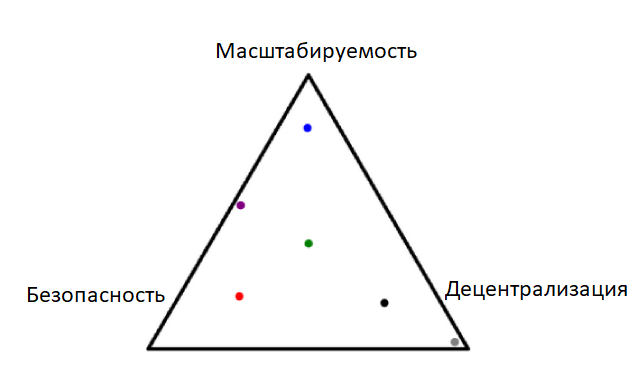
\includegraphics [scale=0.5] {trilem-blockchain}
	\caption{Визуализация трилемммы блокчейна}
	\label{fig:trilem-blockchain}
\end{figure}

Виталик говорит о децентрализации как о возможности запускать блокчейн на таких небольших компьютерах, как ноутбуки, сохраняя при этом безопасность даже в случае проведения атаки с превосходящими мощностями. Таким образом поддерживается устойчивость блокчейна к попытке его изменения, одновременно сохраняя возможность быстро и, что немаловажно, одновременно совершать и обрабатывать большое количество (относительно размера сети) транзакций.

Блокчейны первого поколения (Bitcoin, Ethereum) выбирали безопасность и децентрализацию в ущерб масштабируемости. Когда скорость в 7 транзакций в секунду перестала удовлетворять даже самых преданных фанатов блокчейна, разработчики пытаться прикрутить масштабируемость к тому что есть, в ущерб безопасности. 

Блокчейны следующего поколения слегка отходят от децентрализации. У них не все узлы в сети согласуют свои действия друг с другом, а, например, только 21 очень мощный узел, с высокой пропускной способностью. Так как валидаторов можно сменить путем голосования, сеть всё еще остается децентрализованной. Конечно, 21 компьютер — это не 10 000, как в Биткоине, зато и скорость в среднем достигла 3000 транзакций в секунду.


\section{Постановка задачи} \label{sec:ch1/sec5}
В рамках данной работы требуется провести исследование перспективности применения технологии распределенных реестров для реализации системы электронного документооборота как части инфраструктуры предприятия на примере задачи подписания документов в вузе.

Для этого необходимо реализовать следующие задачи:
\begin{enumerate}
	\item Изучить Enterprise-решение Hyperledger Fabric как систему, реализующую технологию распределенных реестров.
	\item Изучить способы построения надежных систем документооборота.
	\item Реализовать бизнес приложение для системы электронного документооборота.
	\item Реализовать интерфейс взаимодействия с бизнес-приложением на основе REST-API, а также пользовательской части в виде мобильного приложения.
\end{enumerate}

Ключевой аспект системы, разработка которой является одной из задач данной работы, - надежность. Этот аспект назван ключевым, так как в области работы с документами высокая защищенность данных является одной из наиболее необходимых характеристик системы.